\begin{problem}
  Use the triangle given in Figure $1$ to find $\sin (\theta)$, $\cos (\theta)$,
  and $\tan (\theta)$. Provide \textit{exact} values. (The triangle may not be
  drawn to scale.) \textbf{[$5$ points]}

  \begin{figure}[htpb]
    \centering
    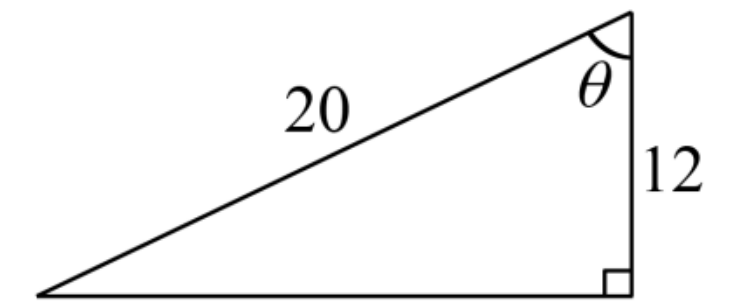
\includegraphics[width=0.8\textwidth]{images/week-6a}
    \caption{}
    \label{fig:}
  \end{figure}
\end{problem}

\begin{solution}
  First, we're going to use the Pythagorean Theorem to find all the missing
  sides.
  \begin{align*}
    \qquad&a^{2} + b^{2} = c^{2} \\
    \implies\qquad&a^{2} + 12^{2} = 20^{2} \\
    \implies\qquad&a^{2} + 144 = 600 \\
    \implies\qquad&a^{2} = 456 \\
    \implies\qquad&\sqrt{a^{2}} = \sqrt{456} \\
    \implies\qquad&a = 2\sqrt{114} \\
  .\end{align*}
  Now, we can solve for the $3$ trig functions.
  \begin{align*}
    \qquad&\sin (\theta) = \frac{\textrm{OPP}}{\textrm{HYP}} \\
    \implies\qquad&\sin (\theta) = \frac{2\sqrt{114}}{20} \\
  .\end{align*}

  So, $\sin (\theta) = \frac{2\sqrt{114}}{20}$

  \begin{align*}
    \qquad&\cos (\theta) = \frac{\textrm{ADJ}}{\textrm{HYP}} \\
    \implies\qquad&\cos (\theta) = \frac{12}{20} \\
    \implies\qquad&\cos (\theta) = \frac{3}{5} \\
  .\end{align*}

  So, $\cos (\theta) = \frac{3}{5}$

  \begin{align*}
    \qquad&\tan (\theta) = \frac{1}{\frac{\textrm{OPP}}{ADJ}} =
      \frac{\textrm{ADJ}}{\textrm{OPP}} \\
    \implies\qquad&\tan (\theta) = \frac{12}{2\sqrt{114}} \\
    \implies\qquad&\tan (\theta) = \frac{6}{\sqrt{114}} \\
  .\end{align*}
  So, $\tan (\theta) = \frac{6}{\sqrt{114}}$
\end{solution}

\newpage

\begin{problem}
  Solve the triangle by finding the missing side $a$ and missing angles $X$ and
  $Y$. (The triangle may not be drawn to scale.) Approximations are acceptable
  here, although they must be denoted correctly. \textbf{[$5$ points]}

  \begin{figure}[htpb]
    \centering
    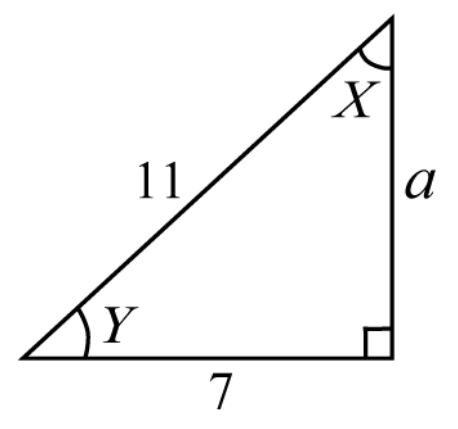
\includegraphics[width=0.8\textwidth]{images/week-6b}
    \caption{}
    \label{fig:}
  \end{figure}
\end{problem}

\begin{solution}
  To solve for $a$, we can use the Pythagorean Theorem:
  \begin{align*}
    \qquad&a^{2} + b^{2} = c^{2} \\
    \implies\qquad&a^{2} + 7^{2} = 11^{2} \\
    \implies\qquad&a^{2} + 49 = 121 \\
    \implies\qquad&a^{2} = 72 \\
    \implies\qquad&\sqrt{a^{2}} = \sqrt{72} \\
    \implies\qquad&a = 6\sqrt{2} \\
  .\end{align*}

  So, $a = 6\sqrt{2}$.

  To find our missing angles, we need to use the inverse functions. First, let's
  solve for $X$:

  \begin{align*}
    \qquad&\tan (Y) = \frac{6\sqrt{2}}{7} \\
    \implies\qquad&\tan^{-1} (\tan (Y)) =
      \tan^{-1} \left(\frac{6\sqrt{2}}{7}\right) \\
    \implies\qquad&Y \approx 0.88 \\
  .\end{align*}

  Now, we can use the $180^{\circ}$ rule to find for $X$:

  \begin{align*}
    \qquad&90 + 0.88 = 90.88 \\
    \implies\qquad&180 - 90.88 = x \\
    \implies\qquad&X \approx 89.12^{\circ}
  .\end{align*}

  So, our final answers are:

  \begin{align*}
    a &= 6\sqrt{2} \\
    X &\approx 89.12^{\circ} \\
    Y &\approx 0.88^{\circ} \\
  .\end{align*}
\end{solution}

\newpage

\begin{problem}
  Solve the triangle by finding the missing side $c$ and missing angles $A$ and
  $B$. (The triangle may not be drawn to scale.) Approximations are acceptable
  here, although they must be denoted correctly. \textbf{[$5$ points]}

  \begin{figure}[htpb]
    \centering
    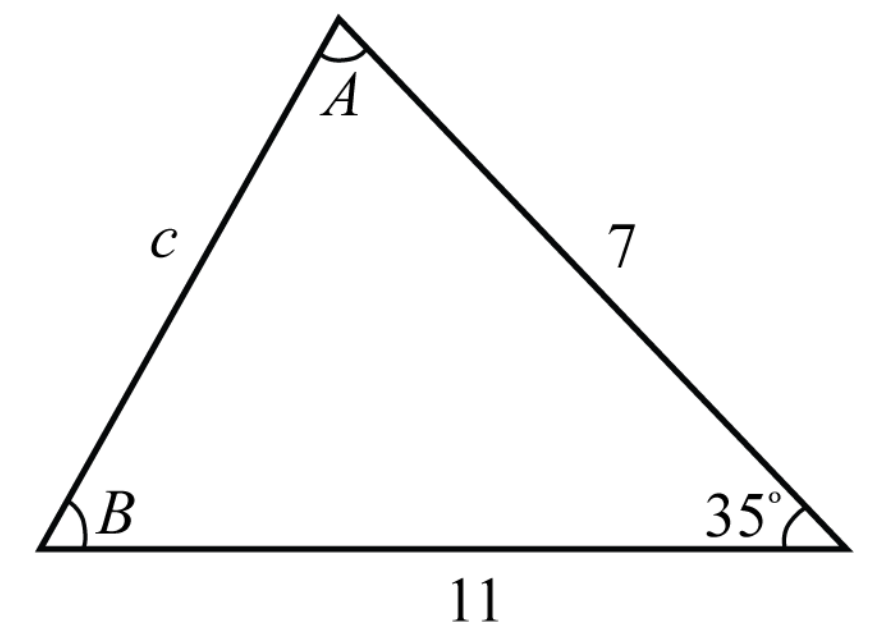
\includegraphics[width=0.8\textwidth]{images/week-6c}
    \caption{}
    \label{fig:}
  \end{figure}
\end{problem}

\begin{solution}
  First, let me solve for $c$.
  \begin{align*}
    \qquad&c^{2} = 11^{2} + 7^{2} - 2(11)(7) \times \cos (35^{\circ}) \\
    \implies\qquad&c^{2} \approx 43.85 \\
    \implies\qquad&\sqrt{c^{2}} \approx \sqrt{43.85} \\
    \implies\qquad&c \approx 6.62 \\
  .\end{align*}

  Now we can use the \textbf{Law of Sines} to find either of the other angles.
  Let's find $B$:

  \begin{align*}
    \qquad&\frac{\sin (B)}{7} = \frac{\sin (35^{\circ})}{c} \\
    \implies\qquad&\sin (B) = \frac{7 \times \sin (35^{\circ})}{c} \\
    \implies\qquad&\sin^{-1} (\sin (B)) =
      \sin^{-1} \left(\frac{7 \times \sin (35^{\circ})}{c}\right) \\
    \implies\qquad&B \approx 37.34 \\ 
  .\end{align*}

  Now we can solve for $A$:

  \begin{align*}
    \qquad&A + B + 35^{\circ} = 180^{\circ} \\
    \implies\qquad&A + 37.34^{\circ} + 35^{\circ} = 180^{\circ} \\
    \implies\qquad&A + 72.34^{\circ} = 180^{\circ} \\
    \implies\qquad&A \approx 107.66^{\circ} \\
  .\end{align*}

  So, here are our final answers:
  \begin{align*}
    A &\approx 107.66^{\circ} \\
    B &\approx 37.34^{\circ} \\
    c &\approx 6.62
  .\end{align*}
\end{solution}
